\section{Theory of Operations}

\subsection{Introduction}
The \textbf{Timer} is a configurable timer module that supports a variety of timing functions, including PWM generation and interrupt signaling. It features a counter that can be configured with a prescaler, maximum count value, and PWM ceiling value.

\begin{figure}[h]
  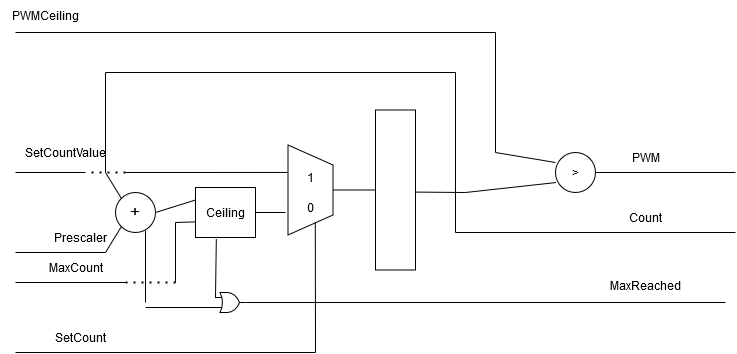
\includegraphics[width=0.80\textwidth]{images/TimerDragram.drawio.png}
  \caption{Timer Diagram}\label{fig:timer-diagram}
\end{figure}

The Timer module provides the following outputs:

\begin{itemize}[noitemsep]
  \item{\textit{count}: Current value of the counter.}
  \item{\textit{maxReached}: Signal indicating the counter has reached its maximum value.}
  \item{\textit{pwm}: PWM output signal with a duty cycle controlled by \textit{pwmCeiling}.}
  \item{\textit{interrupt}: Interrupt signal indicating timer events (e.g., max reached).}
\end{itemize}

\subsection{Interface Timing}
The Timer operates on a synchronous clock and provides outputs that are valid on the rising edge of the clock. The timing diagram below illustrates the behavior of the Timer when the counter reaches its maximum value and generates an interrupt.

% \begin{figure}[h]
%   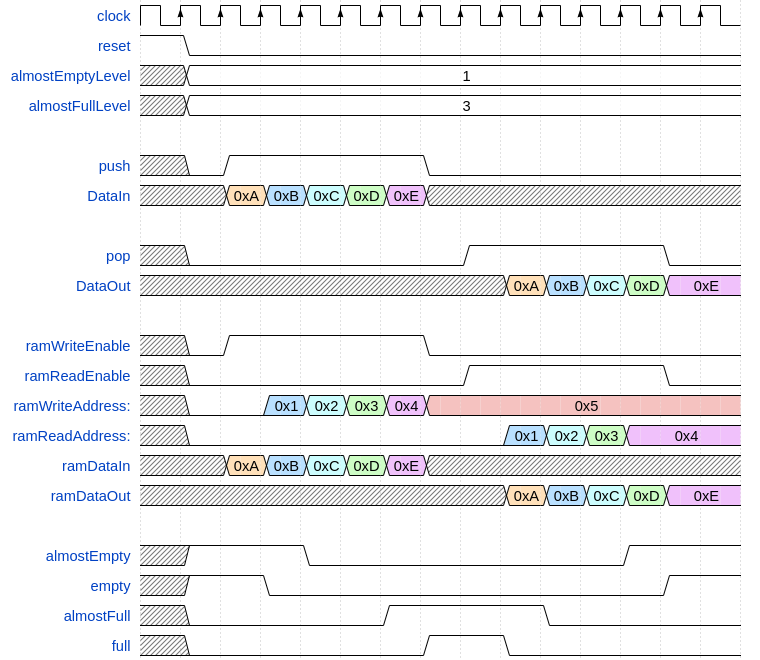
\includegraphics[width=\textwidth]{images/timing.png}
%   \caption{Timing Diagram}\label{fig:timing}
% \end{figure}